% !TEX root = ../thesis.tex

\chapter{Manifold learning techniques\label{ch:ml}}

Since the advent of principal component analysis (PCA) in 1933
\ref{hotelling}, manifold learning has been applied to a wide array of
problems in an effort to unearth hidden structure in data. In a
typical setting, a researcher will collect many data points
$\{x_i\}_{i=1}^N$, often vectors in $\mathbb{R}^n$, that contain
features relevant to the problem under investigation. For example,
when studying collections of $k \times k$-pixel images, it is common
to stack each column of pixel values so that the dataset becomes
vectors $x_i \in \mathbb{R}^n$ where $n = k^2$. Alternatively, when
studying a certain population, each $x_i$ couuld represent a
collection of features about a particular individual such as their
income, education level, and age: a vector in $\mathbb{R}^3$. Manifold
learning would then be applied to this collection of points to reveal
structure in the data that might be obscured by its
high-dimensionality. 

In the latter example, one would expect to find
that income and education level are not indepedent variables, but are
instead positively correlated. This is unsurprising, and hardly a good
use-case for manifold learning. On the other hand, if we study a
collection of images of a human face, each taken at a different angle,
manifold learning can uncover that each image can be described by just
two variables hidden in the dataset: the azimuthal and polar angle at
which the photo was taken \ref{dmaps or isomap}. This example
demonstrates the power of manifold learning as a form of
dimensionality reduction: we can now describe each image as $y_i =
\begin{bmatrix} \theta_i \\ \phi_i \end{bmatrix} \in \mathbb{R}^2$
instead of $x_i \in \mathbb{R}^{4096}$ (if the image contains
$64 \times 64 = 4096$ pixels).  Equivalently, we could say that
$x \in \mathbb{R}^{4096}$ is parameterized by $y = \begin{bmatrix}
  \theta \\ \phi \end{bmatrix} \in \mathbb{R}^2$.

Many approaches have been proposed to address this problem, each
exploiting a different aspect of the dataset. Some are designed to
find linear relationships among input variables \ref{PCA}, others use
the smoothness of the manifold as a basis for a new parameterization
\ref{hessiang eigenmaps}. Below, we detail the mathematical
underpinnings of two particular methods: PCA and Diffusion Maps
(DMAPS). As the most widely used manifold learning technique, PCA is
conceptually simple and provides easily-understandable
results. However, we will see that it is incapable of efficiently
embedding nonlinear manifolds. For this, we turn to DMAPS, a method
that will return a better embedding of the data at the cost of
interpretability. Both are used throughout subsequent sections of this
paper.

\section{Principal component analysis\label{sec:ml:pca}}

In brief, PCA returns a ranking of the important linear relationships
in data. This importance is determined by the amount of the data's
variability a particular linear relationship is able to capture. These
statements are made precise below.

As usual we begin with a collection of $N$ vectors $x_i \in \mathbb{R}^n$,
which we stack in rows to form our input matrix

\begin{align}
  X = \begin{bmatrix} \; - \; x_1^T \; - \; \\ \; - \; x_2^T \; - \; \\ \vdots \\ \; - \; x_N^T
    \; - \; \end{bmatrix} \in \mathbb{R}^{N \times n}
\end{align}

Note that each column represents a particular variable, e.g. age or
income, while each row contains an individual data point. We will
assume that each column has a mean value of zero; if not the mean can
simply be subtracted from each column. We will also assume that we
$N \gg n$, so one imagine can running many experiments in which only a
few variables are measured each time. \\

The problem can now be posed
as: if we projected each $x_i$ along some $v \in \mathbb{R}^n$, which
choice of $v$ would maximize the variance in the projection? More
formally, we wish to solve

\begin{align}
  \max_{v \in \mathbb{R}^n} \mathrm{var}(Xv) = v^TX^TXv \\
  \mathrm{s.t.} \| v \| = 1
\end{align}

where we have added the scaling condition $\| v \| = 1$ to prevent
infinite variances. An equivalent formulation is 

\begin{align}
  \max_{v \in \mathbb{R}^n} \frac{v^TX^TXv}{v^Tv}
\end{align}

where we notice that $\frac{v^TX^TXv}{v^Tv}$ is the Rayleigh quotient
of $M = X^TX$. It is well known that the Rayleigh quotient is
maximized when $v$ is the eigenvector of $M$ corresponding to the
largest eigenvalue. Thus if we order the eigenvalues
$\lambda_1, \lambda_2, \cdots, \lambda_n$ and corresponding
eigenvectors $v_1, v_2, \cdots, v_n$ such that
$\lambda_i \ge \lambda_{i+1}$, we find that $v_1$ is our desired
vector. Note that this makes some intuitive sense as $M = X^TX$ is the
unscaled covariance matrix of $X$, and by choosing the largest
eigenvector of $X^TX$, we are choosing the direction along which
variance is maximized. \\

There is a clear connection between PCA and the singular value
decomposition (SVD) of a matrix, and the two terms are often used
interchangeably. The SVD, which exists for every
$X \in \mathbb{R}^{N \times n}$, is given by

\begin{align}
  X = U D V^T =   
  \begin{bmatrix}
    & & & \\ 
    | & | &  & |  \\
    u_1 & u_2 & \cdots & u_n \\
    | & | &  & |  \\
    & & &  \\
  \end{bmatrix}
  \begin{bmatrix} 
    \sigma_1^2 & & & \\
    & \sigma_2^2 & & \\
    & & \ddots & \\
    & &  & \sigma_n^2 \\
  \end{bmatrix}
  \left[ \begin{array}{ccccc}
           - & \multicolumn{3}{c}{v_1} & - \\
           - & \multicolumn{3}{c}{v_2} & - \\
             & & \vdots & & \\
           - & \multicolumn{3}{c}{v_n} & - \\
         \end{array} \right]
\end{align}

where $U$ and $V$ are $N \times n$ and $n \times n$ unitary matrices,
and $D$ is an $n \times n$ diagonal matrix with non-negative
entries. Now $X^TX$ becomes

\begin{align}
  X^T X = (V D^T U^T) U D V^T = V D^2 V^T
\end{align}

This shows that the vector $v_1$ is the very same vector we desire
from our principal component analysis: the top eigenvector of the
unscaled covariance matrix.

To actually affect any dimensionality reduction, we would use a subset
of these principal components to project our data into some reduced
number of dimensions. For instance, if $\hat{V}$ is an $n \times k$
matrix containing the leading $k$ singular vectors of $X$, we would
have

\begin{align}
  y_i = \hat{V}\hat{V}^T x_i
\end{align}

corresponding to a reduction in dimensionality from $n$ to $k$.

As a concrete example, and to further cement the statistical aspects
of the technique, consider drawing points $x_1$ and $x_2$ from a
multivariate normal distribution. Let them share a mean value of zero
and a variance of one, but let their covariance be two. Thus

\begin{align}
  \mu_1 &= \mu_2 &= 0 \\
  \Sigma_{11} &= \Sigma_{22} &= 4.5 \\
  &\Sigma_{12} &= 5.5
\end{align}

If $\xb = (x_1, x_2)$, $\xb \sim \mathcal{N}(\mub, \Sigma)$ with
$\mub = (\mu_1, \mu_2)$ and $\Sigma = \begin{bmatrix} \sigma_{11}^2 &
  \sigma_{12}^2 \\ \sigma_{12}^2 &
  \sigma_{22}^2 \end{bmatrix}$. Taking the eigendecomposition of
$\Sigma$ we find

\begin{align}
  V = \begin{bmatrix} 1/\sqrt{2} & 1/\sqrt{2} \\
    1/\sqrt{2} & - 1/\sqrt{2} 
  \end{bmatrix} \quad \mathrm{and} \quad
                 \Sigma = \begin{bmatrix} 10 & 0 \\
                   0 & 1 
                 \end{bmatrix}
\end{align}

This, then, would be the expected result of our principal component
analysis: a vector pointing in the $(1,1)$ direction with a
corresponding singular value of $\sqrt{10 n}$, and a second vector pointing in
$(1, -1)$ with singular value $\sqrt{1 n}$ where $n$ is the number of
points in our sample. Fig. \ref{fig:pca-ex} shows a
sample dataset chosen from this particular distribution, along with
principal component vectors scaled by their singular values. The
result is as expected. Indeed, inspecting the numerical output from
5000 points we find

\begin{align}
  V \approx \begin{bmatrix} 1/\sqrt{2} & 1/\sqrt{2} \\
    1/\sqrt{2} & - 1/\sqrt{2} 
  \end{bmatrix} \quad \mathrm{and} \quad
                 \Sigma = \begin{bmatrix} 222 \approx \sqrt{50000} & 0 \\
                   0 & 71 \approx \sqrt{5000}
                 \end{bmatrix}
\end{align}

\begin{figure}
  \centering
  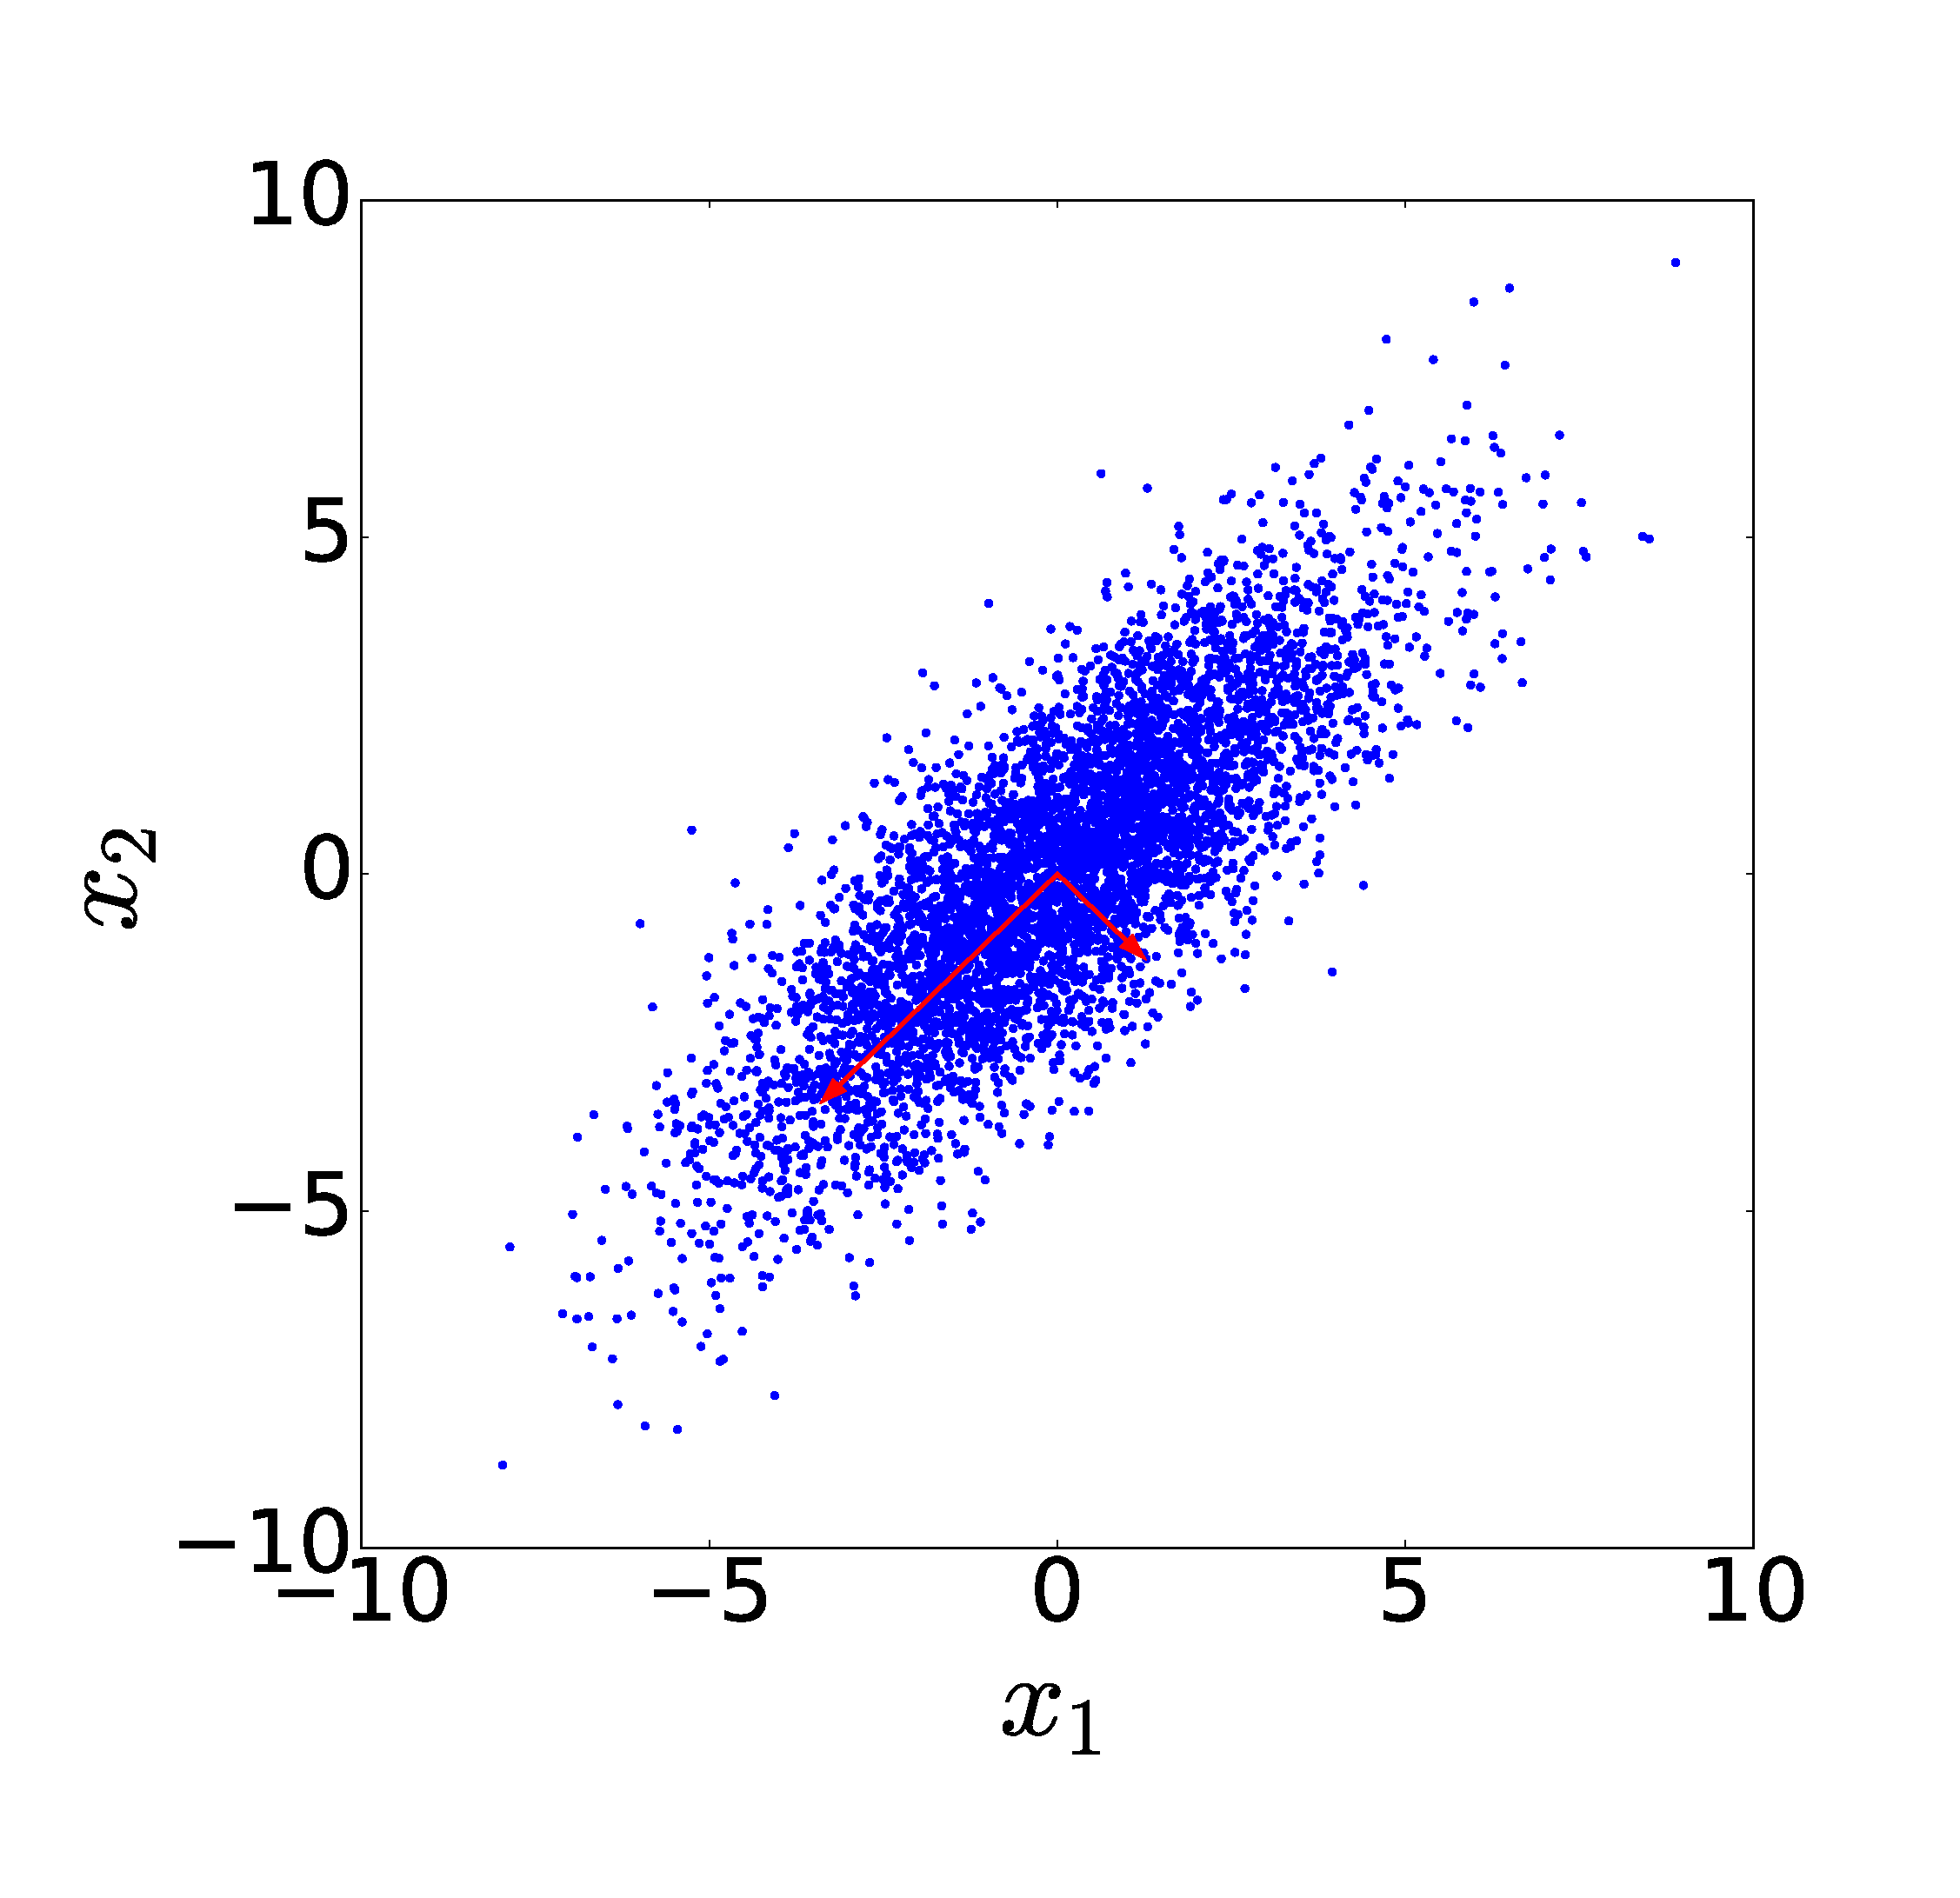
\includegraphics[width=0.8\textwidth]{pca-ex}
  \caption{Principal components found through PCA on the blue point
    cloud, scaled by singular value. \label{fig:pca-ex}}
\end{figure}

Besides its relative simplicity and ease of implementation, PCA has
one other great strength compared to other dimensionality reduction
methods: it provides an explicit functional form between the input
variables and the output projection in the form of a simple, linear
relationship. In the context of PCA, the principal vectors, which are
some linear combination of the input variables, are precisely the
``best'' new variables to work in. Using the output of the previous
example, we may decide that only the value $x_1 + x_2$ is important
enough to keep, allowing us to reduce our description of the dataset
from $(x_1, x_2) \rightarrow (x_1 + x_2)$. As we will see in the
following section, while more complex methods offer distinct
advantages over PCA, they lack such easily interpretable results.

\section{Diffusion Maps \label{sec:dmaps}}

While PCA may be effective in uncovering linear relationships among
input variables, most real-world problems exhibit significant
nonlinearities. This motivates our introduction of Diffusion Maps
(DMAPS), an algorithm designed to address such difficulties. We begin
with a description of the DMAPS' implementation.

The goal of DMAPS is identical to that of PCA: given some dataset
$\{x_1, x_2, \hdots, x_N \}$ with $x_i \in \R^n$, we desire a mapping
of $x_i$ into $y_i$ such that $y_i$ is a low-dimensional embedding of
$x_i$ that captures important characteristics of the original data. We
again stack each datapoint $x_i$ into an $N \times n$ matrix
$X$. DMAPS begins by evaluating a Gaussian kernel between each point,
and storing the results in an $N \times N$ matrix $W$, so that

\begin{align}
  W_{ij} = \exp \left( -\frac{\|x_i - x_j\|^2}{\epsilon^2} \right)
\end{align}

where $\epsilon$ is a parameter which will be discussed below. Note
that $W_{ij} \rightarrow 0$ as the distance between $x_i$ and $x_j$
increases. We then calculate the sum of each row of $W$, and use these
values to construct a new diagonal matrix $D$ with
$D_{ii} = \sum_j W_{ij}$. Finally, we compute $A = D^{-1} W$. As
$A_{ij} \ge 0$ and $\sum_j A_{ij} = 1$, $A$ is a stochastic
matrix. This lends its entries $A_{ij}$ an intuitive interpretation:
if we are performing a random walk from point to point in our dataset,
$A_{ij}$ is the probability that, starting from $x_i$ we will hop next
to $x_j$. Just as $W_{ij}$ decreases when the distance between $x_i$
and $x_j$ grows, so too will $A_{ij}$ decrease, so that the
probability of jumping to nearby points is much greater than the
probability of jumping to distant ones. This concept is illustrated in
Fig.~\ref{fig:dmaps-3pts} for three points.

\begin{figure}
  \centering
  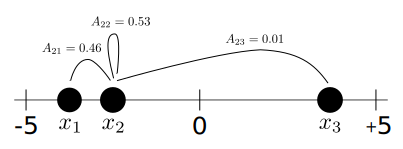
\includegraphics[width=0.8\textwidth]{dmaps-3pts}
  \caption{Probability of transitioning from $x_1$ to points $x_2$ and
    $x_3$ and to itself. \label{fig:dmaps-3pts}}
\end{figure}
